\begin{frame}[fragile]{What is a destabilizing attack? (and why you should care?)}

%\vspace{-0.045in}

\begin{center}
\begin{tikzpicture}[scale=0.9]
\small

%\draw[blue,line width=0.25pt,fill,draw opacity=0.5,fill opacity=0.1]
    %(-3.95,0.8) -- (-2.75,0.8) -- (-2.75,1.9) -- (-3.95,1.9) -- cycle;
    %(-4.85,0.8) -- (-3.65,0.8) -- (-3.65,1.9) -- (-4.85,1.9) -- cycle;

%\draw[dotted,thick] (-3.95,1.9) -- (-4.1,3.6);
%\draw[dotted,thick] (-2.75,1.9) -- (4.1,3.6);

\node[rectangle,align=center] at (4,-0.75) {standard IEEE \\ 9 bus power system};
\uncover<2>{
\node at (4,-1.5) { (\textcolor{darkgreen}{normal operations}) };
}
\uncover<3>{
\node at (4,-1.5) { (\textcolor{red}{static attack}) };
}
\uncover<4-7>{
\node at (4,-1.5) { (\textcolor{red}{dynamic attack}) };
}

%\node[rectangle,align=center] at (5.2 ,4.8) {\rotatebox{90}{Rotor Angle}};
%\node[rectangle,align=center] at (4.85,4.8) {\rotatebox{90}{Frequency}};
%\node[rectangle,align=center] at (4.5 ,4.8) {\rotatebox{90}{Deviation}};

\uncover<2-7>{
\node[rectangle,align=center] at (5.5 ,6.0) {\color{blue} rotor angle};
\node[rectangle,align=center] at (5.5 ,5.55) {\color{blue} frequency};
\node[rectangle,align=center] at (5.5 ,5.10) {\color{blue} deviation};

\node[rectangle,align=center] at (5.95 ,3.50) {\color{purple} bus load (kW)};

%\node at (0,10) {};
\node at (0,5.5) {
    \begin{tikzpicture}[scale=0.9]

    \draw[fill=green,draw opacity=0,fill opacity=0.05] (0,0.3) -- (8.20,0.3) -- (8.20,1.95) -- (0,1.95);
    \draw[dashed,darkgreen] (0,0.3) -- (8.2,0.3);
    \draw[dashed,darkgreen] (8.2,1.95) -- (0,1.95);

    \node at (3.25,0.5) {\color{darkgreen} safe operating range};
    \uncover<2>{
    \begin{axis}
        [ domain=-30:80
        , xmin=-30
        , xmax=80
        , ymin=-2000
        , ymax=2000
        , width=3.85in
        , height=1.5in
        , samples=500
        , xtickmin=1,xtickmax=0,ytickmin=1,ytickmax=0, minor tick num=0, scaled ticks=false, xticklabel=\empty,yticklabel=\empty
        ]
    \draw[ultra thin,opacity=0.2] (axis cs:\pgfkeysvalueof{/pgfplots/xmin},0) -- (axis cs:\pgfkeysvalueof{/pgfplots/xmax},0);
    \addplot[color=blue,mark=none] {0};
    \end{axis}
    }
    \uncover<3>{
    \begin{axis}
        [ domain=-30:80
        , xmin=-30
        , xmax=80
        , ymin=-2000
        , ymax=2000
        , width=3.85in
        , height=1.5in
        , samples=500
        , xtickmin=1,xtickmax=0,ytickmin=1,ytickmax=0, minor tick num=0, scaled ticks=false, xticklabel=\empty,yticklabel=\empty
        ]
    \draw[ultra thin,opacity=0.2] (axis cs:\pgfkeysvalueof{/pgfplots/xmin},0) -- (axis cs:\pgfkeysvalueof{/pgfplots/xmax},0);
    \addplot[color=blue,mark=none] {(\x>0)*2000*(x/4)^(0.5)*exp(-(x/4)^(1.5))};
    \end{axis}
    }
    \uncover<4-7>{
    \begin{axis}
        [ domain=-30:80
        , xmin=-30
        , xmax=80
        , ymin=-2000
        , ymax=2000
        , width=3.85in
        , height=1.5in
        , samples=500
        , xtickmin=1,xtickmax=0,ytickmin=1,ytickmax=0, minor tick num=0, scaled ticks=false, xticklabel=\empty,yticklabel=\empty
        ]
    \draw[ultra thin,opacity=0.2] (axis cs:\pgfkeysvalueof{/pgfplots/xmin},0) -- (axis cs:\pgfkeysvalueof{/pgfplots/xmax},0);
    \addplot[color=blue,mark=none] {(\x>0)*x^(1.75)*sin(deg(x))};
    \end{axis}
    }

    \end{tikzpicture}
};
\node at (0,3.5) {
    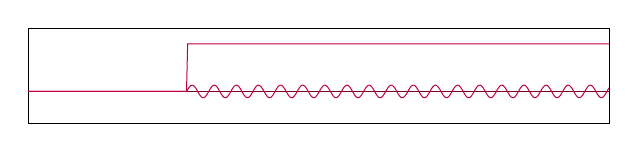
\begin{tikzpicture}[scale=0.9]
    \uncover<2>{
    \begin{axis}
        [ domain=-30:80
        , xmin=-30
        , xmax=80
        , ymin=-1000
        , ymax=2000
        , width=3.85in
        , height=1.15in
        , samples=500
        , xtickmin=1,xtickmax=0,ytickmin=1,ytickmax=0, minor tick num=0, scaled ticks=false, xticklabel=\empty,yticklabel=\empty
        ]
    \draw[ultra thin,opacity=0.2] (axis cs:\pgfkeysvalueof{/pgfplots/xmin},0) -- (axis cs:\pgfkeysvalueof{/pgfplots/xmax},0);
    \addplot[color=purple,mark=none] {0};
    \end{axis}
    }
    \uncover<3>{
    \begin{axis}
        [ domain=-30:80
        , xmin=-30
        , xmax=80
        , ymin=-1000
        , ymax=2000
        , width=3.85in
        , height=1.15in
        , samples=500
        , xtickmin=1,xtickmax=0,ytickmin=1,ytickmax=0, minor tick num=0, scaled ticks=false, xticklabel=\empty,yticklabel=\empty
        ]
    \draw[ultra thin,opacity=0.2] (axis cs:\pgfkeysvalueof{/pgfplots/xmin},0) -- (axis cs:\pgfkeysvalueof{/pgfplots/xmax},0);
    \addplot[color=purple,mark=none] {(\x>0)*1500};
    \end{axis}
    }
    \uncover<4-7>{
    \begin{axis}
        [ domain=-30:80
        , xmin=-30
        , xmax=80
        , ymin=-1000
        , ymax=2000
        , width=3.85in
        , height=1.15in
        , samples=500
        , xtickmin=1,xtickmax=0,ytickmin=1,ytickmax=0, minor tick num=0, scaled ticks=false, xticklabel=\empty,yticklabel=\empty
        ]
    \draw[ultra thin,opacity=0.2] (axis cs:\pgfkeysvalueof{/pgfplots/xmin},0) -- (axis cs:\pgfkeysvalueof{/pgfplots/xmax},0);
    \addplot[color=purple,mark=none] {(\x>0)*200*sin(deg(1.5*x))};
    \end{axis}
    }
    \end{tikzpicture}
};
}

\node at (0,0) {
    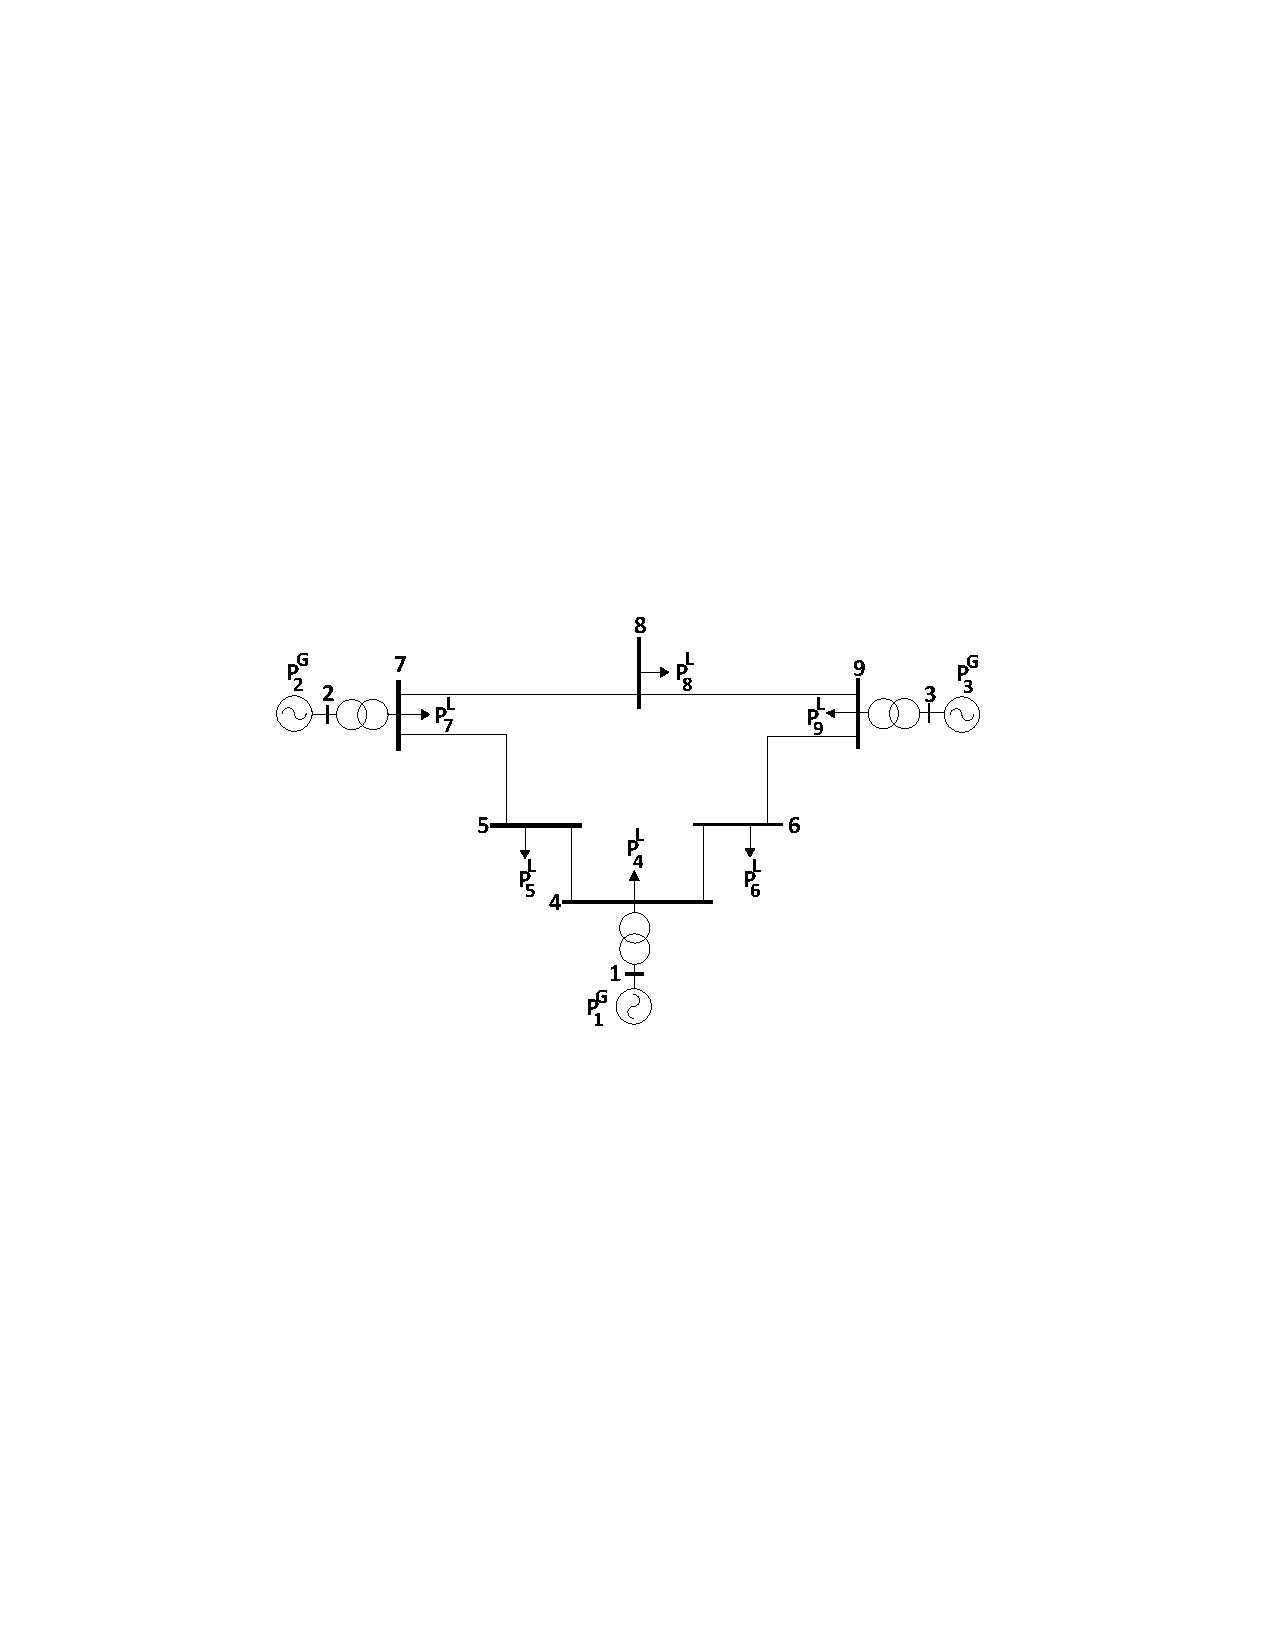
\includegraphics[width=2.7in]{img/IEEE9}
    %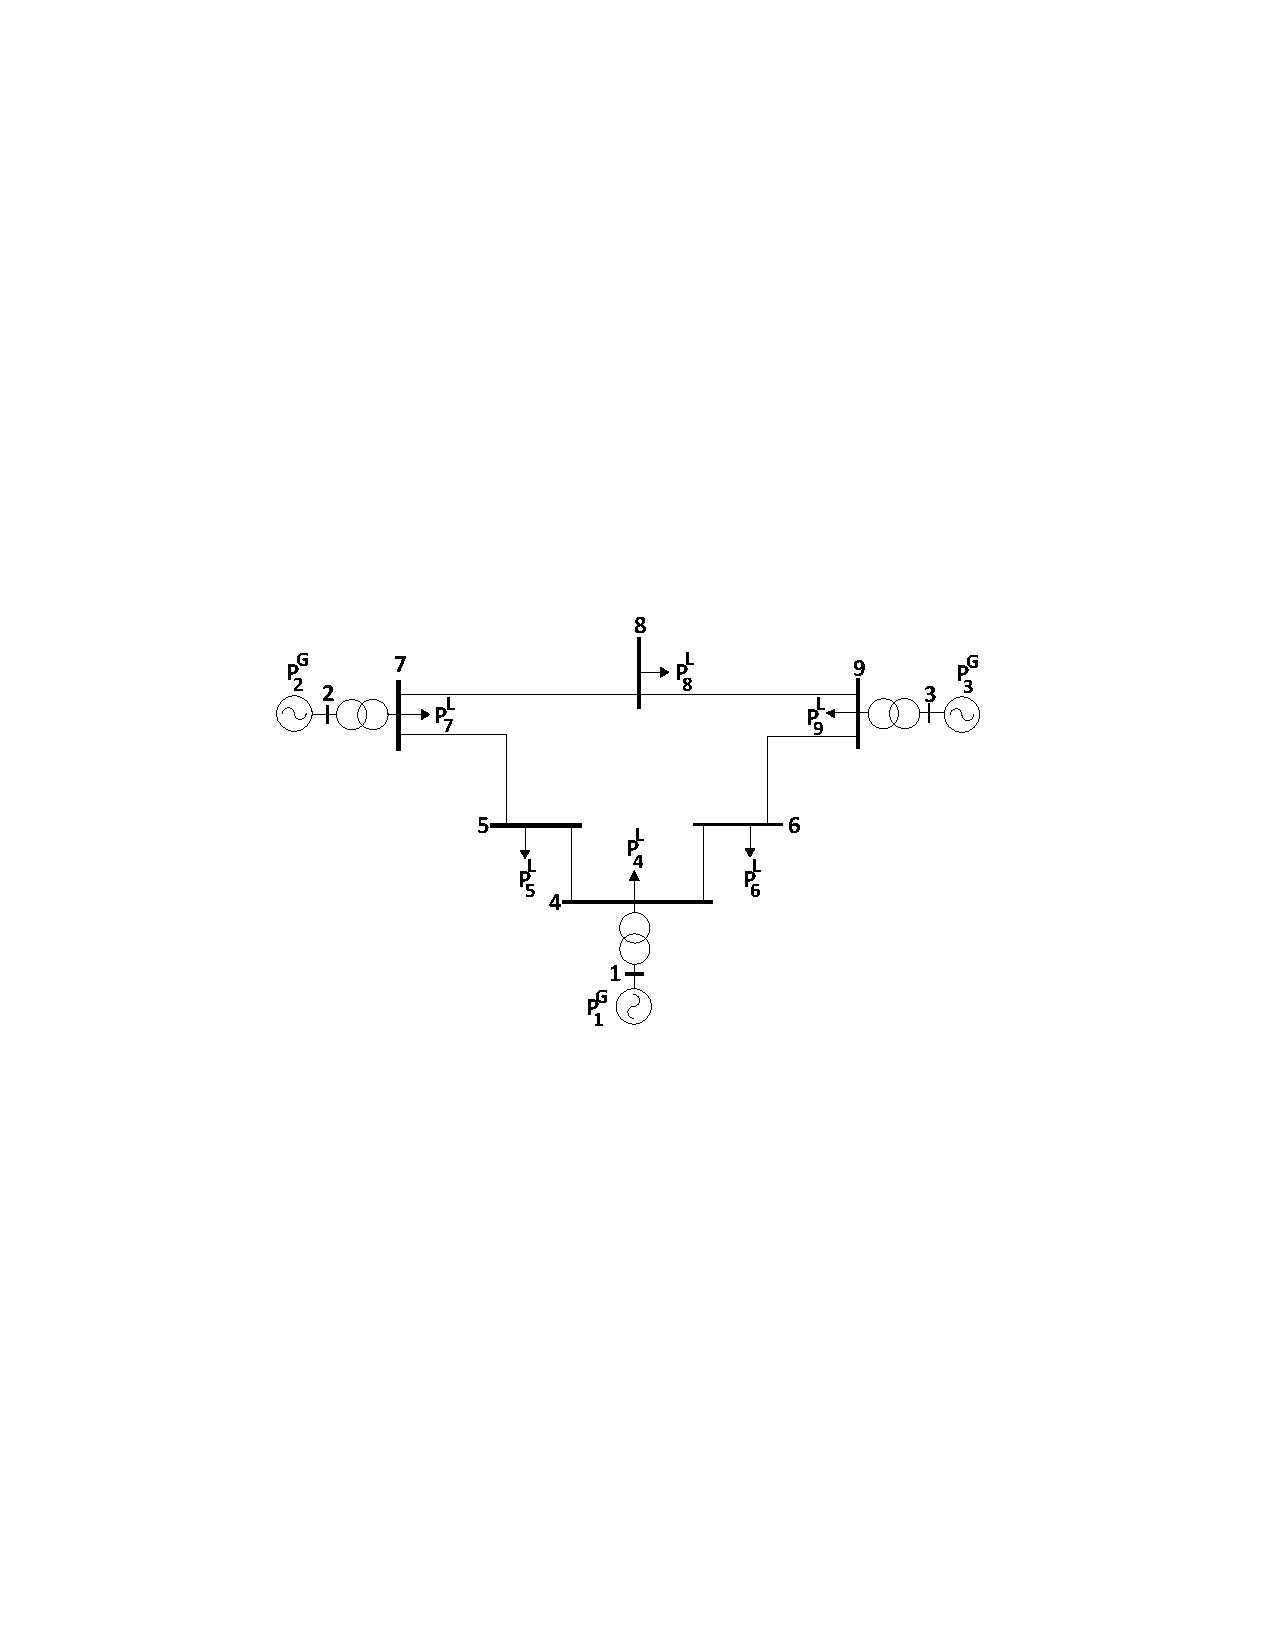
\includegraphics[width=3in]{img/IEEE9}
    %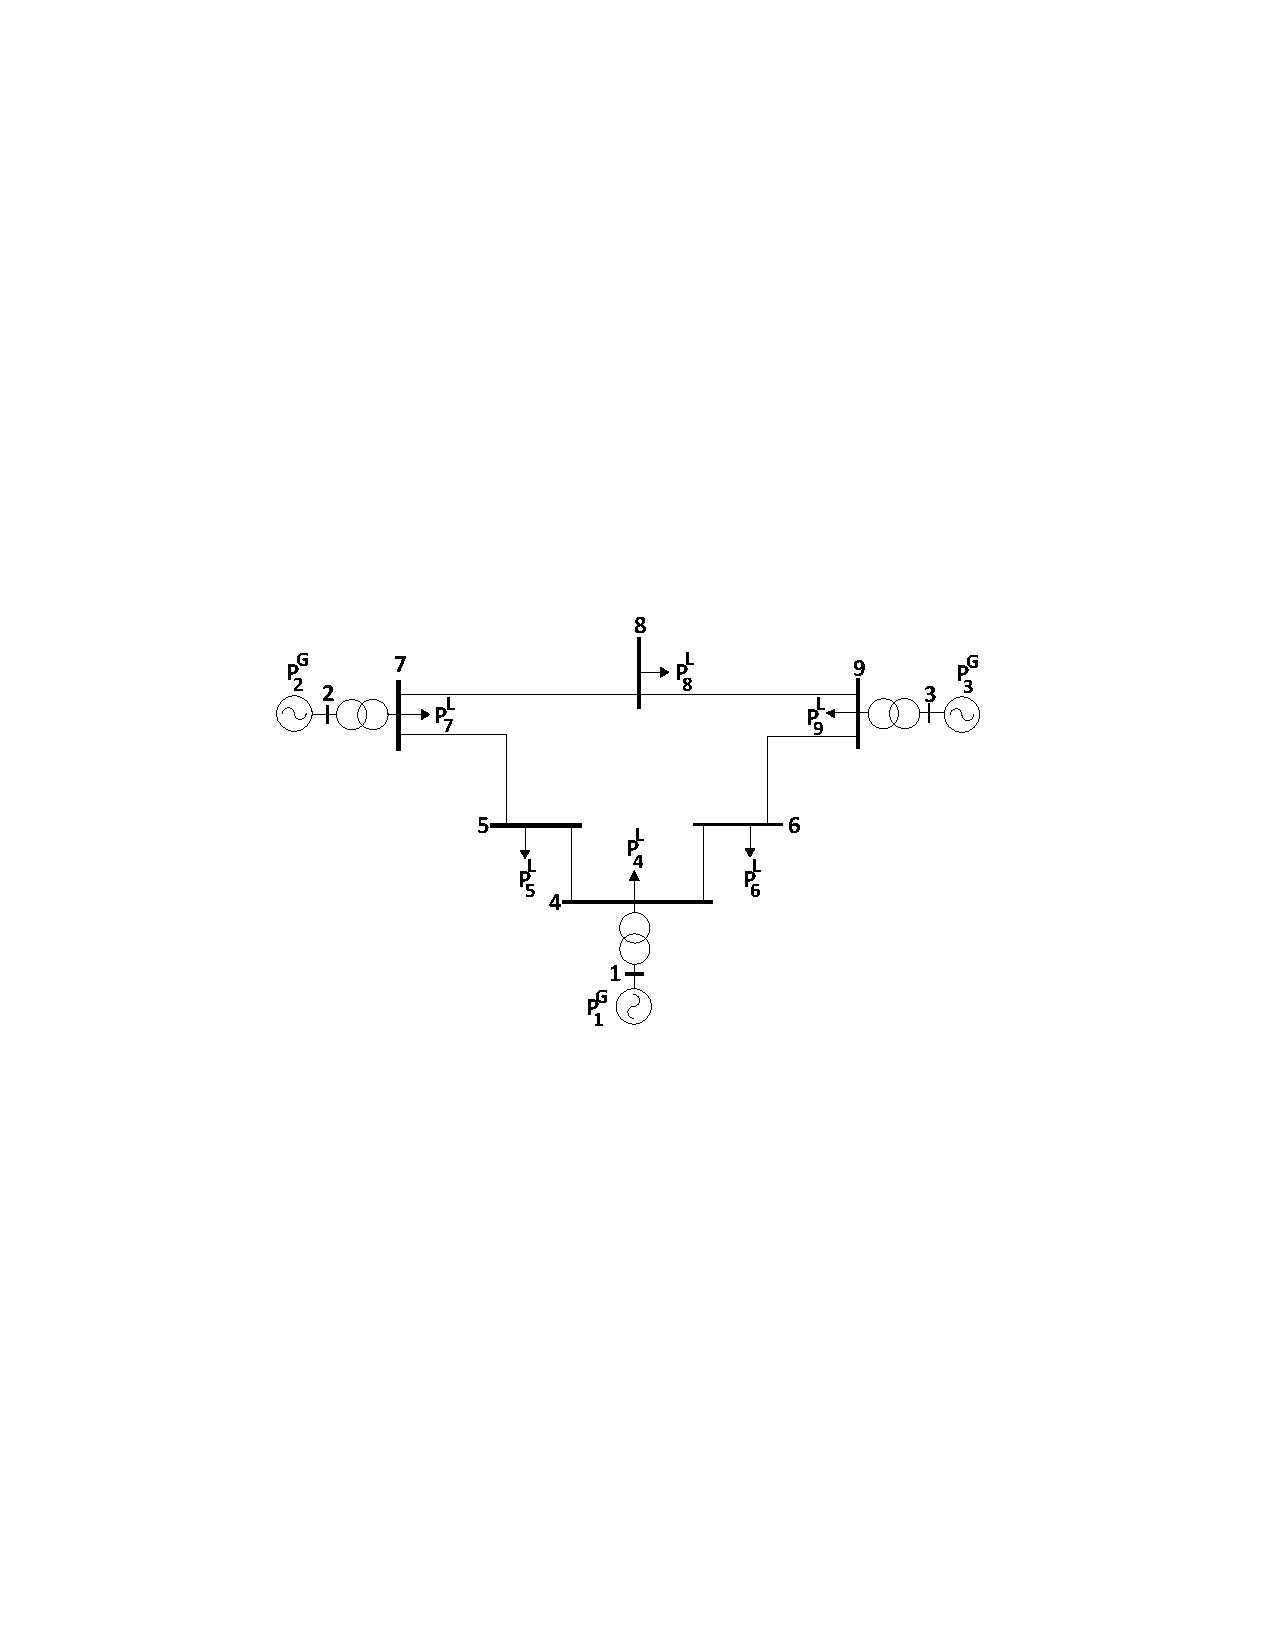
\includegraphics[width=0.8\textwidth,height=1.7in]{img/IEEE9}
};

\uncover<2-7>{
\node[draw=purple,fill=purple,fill opacity=0.05,circle,minimum width=1.5cm] (8) at (0.25,1.6) {};
\draw[->,draw=purple,thick] (-0.55,1.8) to[in=270,out=150] (-1.5,2.75);

\node[draw=blue,fill=blue,fill opacity=0.05,circle,minimum width=1.5cm] at (-3.25,1.25) {};
\draw[->,draw=blue,thick] (-4.05,1.6) to[in=225,out=150] (-4.25,5.25);
}

\uncover<5-7>{
\node[draw=red,fill=red,fill opacity=0.05,circle,minimum width=1.5cm] (3) at (3.5,1.25) {};
\draw[red,thick,->] (3) to[out=120,in=20] (8);

\node[rectangle,align=center] at (5.25,1) {\color{red}positive \\\color{red}feedback};
%\node at (4,-0.35) {\color{red}between unrelated nodes};
}

\uncover<6-7>{
\node[minimum width=4.55in,minimum height=0.5in,draw=blue,rectangle,rounded corners=0.5cm,fill=white] at (0.25in,-0.8) {};
\node[minimum width=4.55in,minimum height=0.5in,draw=blue,rectangle,rounded corners=0.5cm,fill=blue,opacity=0.05] at (0.25in,-0.8) {};
}
\uncover<6>{
\node[minimum width=4.55in,minimum height=0.5in,draw=blue,rectangle,rounded corners=0.5cm,align=left] at (0.25in,-0.8) 
    { \normalsize \textbf{Previous work:} detects the presence of an attack 
    };
}
\uncover<7>{
\node[minimum width=4.55in,minimum height=0.5in,draw=blue,rectangle,rounded corners=0.5cm,align=left] at (0.25in,-0.8) 
    { \normalsize \textbf{Our work:} identify which bus is attacked (so we can isolate it)
    };
}


\end{tikzpicture}
\end{center}

\end{frame}

